\section{Experiment 1: Comparative Enlarged Figure-Eight Evaluation}
The public project contains exactly two main experiments. Historical model validations and the earlier PPO campaign above provide context, not additional primary experiments. Experiment1 compares native tracking at $A=0.75$ m, $B=0.375$ m and $T=30$ s on the unchanged $2$ mm rough terrain. Three paired reset/terrain contexts are used. V4 and PPO traces are reused with preserved hashes; V2, V3, V2\_FFv1 and V3\_FFv1 receive twelve new native trials. Physical parameters, initial states, torque bounds, reference and original sixteen-window metrics remain fixed. Privileged liquid-state methods are identified separately. PID, teacher and mixture-policy variants without a verified equivalent release interface are explicitly not evaluated.

\begin{table}[ht]\centering\caption{Experiment1 outcomes across three matched contexts. Full duration alone is not task success.}\begin{tabular}{lcc}\hline Method & Full30s & Full task\\\hline
PPO & 3/3 & 0/3\\
V2 & 0/3 & 0/3\\
V2\_FFv1 & 0/3 & 0/3\\
V3 & 0/3 & 0/3\\
V3\_FFv1 & 3/3 & 0/3\\
V4 & 3/3 & 0/3\\
\hline\end{tabular}\end{table}
Position-only V2/V3 encounter the original tracking guard near $1.3$--$1.4$ s. V2\_FFv1 reaches the ROM guard at approximately $20$--$24$ s. V3\_FFv1 completes the duration but has roughly $85$--$89$ degrees of yaw drift and only fifteen windows. V4 and PPO retain fifteen windows. No method solves the complete task. Failed-prefix energy is never ranked as a full-horizon sloshing improvement. These are controller-and-information comparisons, not an information-matched causal ranking of algorithms.

\begin{figure}[ht]\centering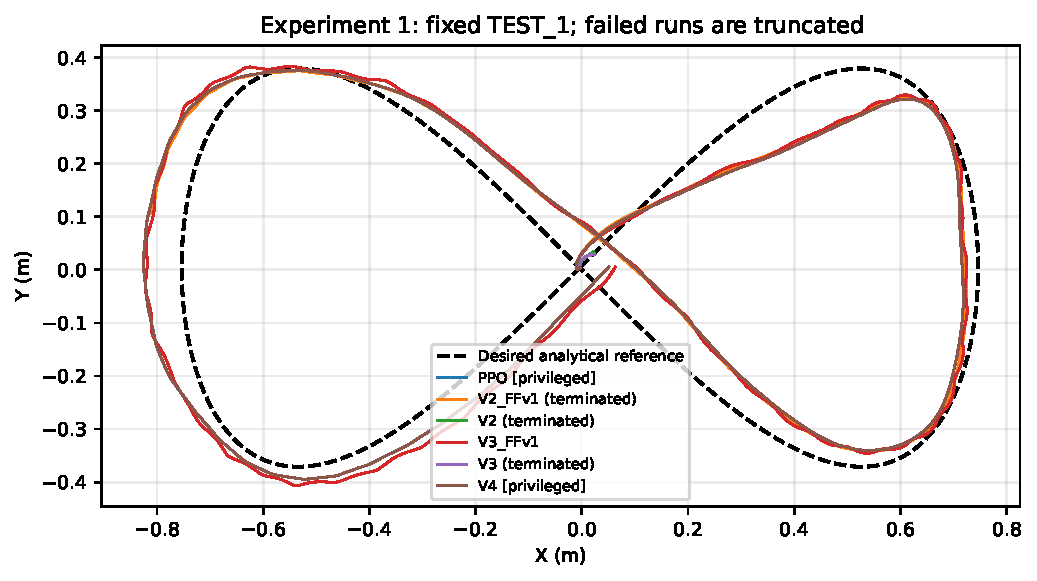
\includegraphics[width=.95\linewidth]{../assets/plots/experiment_1/trajectory.pdf}\caption{Actual native paths for the fixed first context. Failed trials stop at their recorded prefixes.}\end{figure}

\section{Experiment 2: Commanded Navigation and Balance Stability}
A separate $4\times4$ m collision heightfield contains a flat initialization disk, mild roughness, smooth uneven terrain and two small raised features. The scientific benchmark heightfield is unchanged. Arrow keys request bounded forward velocity and yaw rate; a separately named feedforward/heading adapter produces world position, velocity, acceleration and heading targets for stabilizing control. Velocity, yaw-rate and slew bounds are $0.04$ m/s, $0.08$ rad/s, $0.04$ m/s$^2$ and $0.08$ rad/s$^2$. No key directly requests motor torque. Key release, focus loss and stop request return to neutral through the slew limits. GLFW implements pause, reset, cameras and exit, with timestamped input and native telemetry.

The fixed sixteen-second command sequence covers idle, forward, stop, reverse, left/right turns and neutral. Two of three baseline contexts pass; one reaches the ROM guard near $11.986$ s at small tilt. A separately registered twenty-six-second route travels farther and passes in all three contexts, reaching about $0.72$ m radius and visiting flat, transition, mild-rough and smooth-uneven regions. Raised features are not certified by these paths. These contrasting outcomes demonstrate command dependence rather than general robustness.

One controlled diagnostic adds unchanged frozen modal feedback to the same motion adapter. This privileged backbone transfer passes the first standard context but reaches the ROM guard in the second. The third and extended modal trials are gated off, and the variant is not promoted as an improved controller. The plant, fluid damping, gains and safety thresholds are not retuned.

Metrics include roll/pitch RMS, maximum tilt, velocity/yaw-rate tracking error, torque, modal energy/displacement, contact validity, completion and failure time. Recovery requires speed error at most $0.015$ m/s, yaw-rate error at most $0.04$ rad/s and tilt at most $0.06$ rad for $0.5$ s before the next command; intervals without settlement are censored. A two-second automated GUI smoke measured approximately $25.5$ rendered frames/s and near-unity simulated/wall time; no sustained real-time or human-driving claim follows.

\begin{figure}[ht]\centering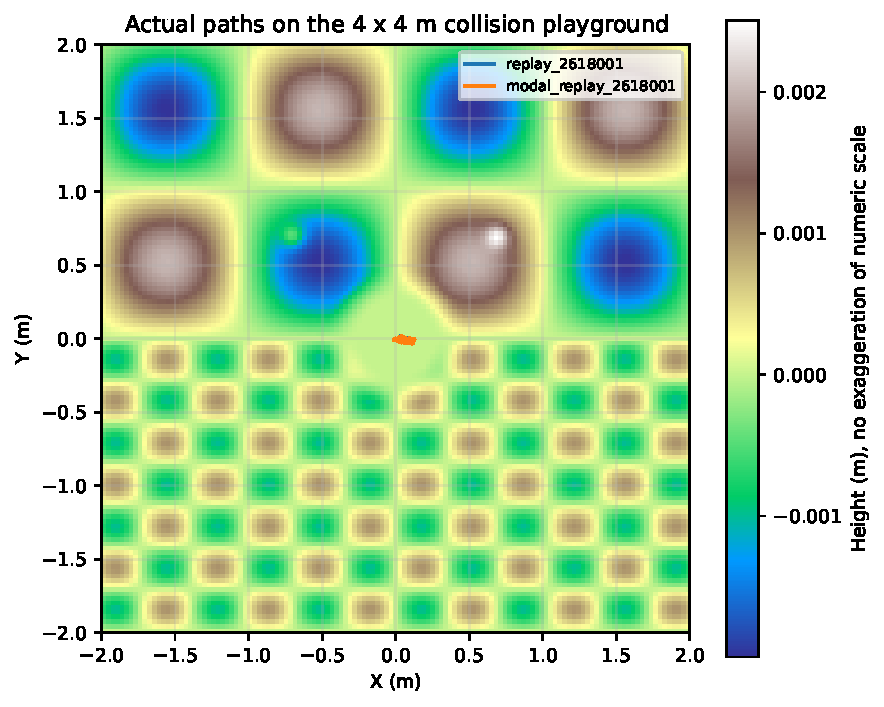
\includegraphics[width=.95\linewidth]{../assets/plots/experiment_2/terrain_path.pdf}\caption{Recorded closed-loop paths on the new collision playground. Successful route coverage does not validate unvisited zones.}\end{figure}

\section{Release and Scientific Boundaries}
The clean export retains source/model provenance, the original license, frozen checkpoint, raw trials, tests, scientific figures and native replay videos. Replay videos integrate no physics and fabricate no fluid surface. Some original observer-guard failures end their stored trace one native interval before termination; these are explicitly labeled, and the later diagnostic revision additionally stores terminal native states. The liquid remains a modal approximation with SPH\_BLOCKED status. One PPO lineage, three contexts and disclosed recovery/seed deviations do not establish broad policy superiority. No hardware validation, full fluid validation or GitHub publication is claimed.

\paragraph{Heightfield representation audit.} Final release QC found that unvisited raised features exceeded the nominal normalized heightfield range. The application now recompiles its temporary terrain representation to keep samples in $[0,1]$, preserving physical world heights within the native float32 quantization bound and leaving robot/liquid parameters unchanged. A new three-second pilot and one-second GUI smoke pass; the completed sixteen- and twenty-six-second results remain explicitly pre-fix. They are not reclassified as long-horizon certification of the corrected representation or of the raised features.
